% Compile from this directory: xelatex -interaction=nonstopmode TokenTrail_Project_Outline.tex
\documentclass[11pt,a4paper]{article}
\usepackage[margin=16mm,top=16mm,bottom=16mm]{geometry}
\usepackage{fontspec,graphicx,tabularx,booktabs,array,enumitem,hyperref,tikz}
\usepackage[table]{xcolor}
\usetikzlibrary{positioning,arrows.meta}
\setmainfont{msyh.ttc}[Path={/Applications/Microsoft Word.app/Contents/Resources/DFonts/},BoldFont=msyhbd.ttc,AutoFakeSlant=0.2]
\setsansfont{msyh.ttc}[Path={/Applications/Microsoft Word.app/Contents/Resources/DFonts/},BoldFont=msyhbd.ttc,AutoFakeSlant=0.2]
\definecolor{navy}{HTML}{315E75}
\definecolor{teal}{HTML}{2E766E}
\definecolor{amber}{HTML}{A17431}
\definecolor{lightblue}{HTML}{EAF3F7}
\definecolor{lightteal}{HTML}{EDF6F2}
\definecolor{lightamber}{HTML}{FAF3E5}
\definecolor{lightrow}{HTML}{F7FAFB}
\definecolor{hairline}{HTML}{BDD0D8}
\arrayrulecolor{navy}
\hypersetup{colorlinks=true,urlcolor=black,linkcolor=black,pdftitle={TokenTrail Project Outline}}
\setlength{\parindent}{0pt}
\setlength{\parskip}{4pt}
\setlist[itemize]{leftmargin=17pt,itemsep=2pt,topsep=3pt}
\renewcommand{\arraystretch}{1.19}
\newcolumntype{Y}{>{\raggedright\arraybackslash}X}
\newcommand{\sect}[1]{\vspace{5pt}{\large\bfseries#1}\par\vspace{2pt}}
\newcommand{\smallhead}[1]{{\bfseries#1}}
\newcommand{\tagline}[1]{\colorbox{lightblue}{\parbox{\dimexpr\linewidth-2\fboxsep}{#1}}}
\pagestyle{plain}
\begin{document}
\color{black}

{\fontsize{22}{26}\selectfont\bfseries TokenTrail}\hfill{\normalsize Android App Project Outline}\par
\vspace{3pt}{\color{navy}\hrule height 0.7pt}\vspace{4pt}
\textbf{Category:} Developer Productivity / API Cost Analytics\hfill\textbf{Target users:} API-key agent users.

\sect{1. App idea and user problem}
TokenTrail is an Android API-cost companion for students and independent developers who use API-key coding agents: \textbf{Codex with OpenAI}, \textbf{ZCode with general Z.ai API access} and a DeepSeek-side tool to be selected. A small pet floats \textbf{within TokenTrail's screens}; tapping it opens an expandable question panel. This \textbf{advice agent} explains cost changes or suggests a coding agent using logged usage, budgets and task ratings. TokenTrail \textbf{does not run, route or control} the coding agents.

The scope is \textbf{API usage priced at public API rates}; ChatGPT or GLM Coding Plan subscriptions and credits are excluded. A model response reports tokens for one call, not the agent's full history. TokenTrail imports available usage logs and prices a call only when a saved official-rate snapshot covers its date; otherwise historical cost is unavailable. An API key alone cannot recover another Agent's past per-call usage. Every monetary value is labelled an \emph{estimate}, never an invoiced charge.

\sect{2. Related products and opportunity}
The review compares first-party API billing views with existing cross-model monitoring tools on data scope, cost provenance and decision support.\par
\begin{tabularx}{\linewidth}{@{}>{\raggedright\arraybackslash}p{27mm}Y Y@{}}
\toprule
\rowcolor{lightblue}
\textbf{Product} & \textbf{Relevant capability} & \textbf{Gap addressed by TokenTrail} \\
\midrule
\href{https://learn.chatgpt.com/docs/auth}{Codex} & Can run with an OpenAI API key, billed through the Platform account. & TokenTrail estimates only logged Codex API calls using dated OpenAI prices. \\
\rowcolor{lightrow}
\href{https://zcode.z.ai/en/docs/configuration}{ZCode} & Can use the general Z.ai API endpoint with an API key, separate from Coding Plan. & TokenTrail prices logged general-API calls, excluding plan usage. \\
\href{https://github.com/bowenliang123/dsh-context/blob/main/README.md}{dsh-context} & DeepSeek Harness plugin showing local sessions, token use, cache, activity and estimated costs. & TokenTrail spans API providers; session detail appears only when usable logs are imported. \\
\rowcolor{lightrow}
\href{https://docs.litellm.ai/docs/simple_proxy}{LiteLLM} & Open-source gateway with routing, spend tracking and budgets for proxied calls. & TokenTrail does not proxy traffic; it tracks agent-associated API costs from permitted records. \\
\href{https://github.com/zhu1090093659/dsh-pet/blob/main/README.zh.md}{dsh-pet} & Interactive floating pet driven by DSH session events, with touch and feeding actions. & TokenTrail adds cross-provider, evidence-linked advice through an Android in-app pet. \\
\bottomrule
\end{tabularx}
\sect{3. Proposed contribution}
\textbf{Unified view.} TokenTrail unifies authorised API-call logs from Codex, ZCode and a DeepSeek-side tool, de-duplicates records and shows their source and coverage; session detail appears only where logs support it. \textbf{Reproducible costs.} Java applies dated official rates by provider, model, token class and service tier, retaining the price version behind each estimate when rates change. \textbf{Decision support.} Activity, budgets and ratings of comparable tasks help users understand spending and choose an agent. The in-app floating pet is the conversational interface: read-only tools supply calculated evidence, and the model explains advice with sample size and missing-data limits. It neither controls coding agents nor encourages extra token use. Values remain \emph{Estimated}, \emph{Partial estimate} or \emph{Unavailable}.

\tagline{\textbf{Scope rule:} API-cost records, comparisons and the in-app advice pet are core. The pet can recommend but cannot execute coding agents or enforce a hard cap. Subscription quotas, public community, live cross-Agent status and system-wide overlays are outside the first release.}

\newpage
\sect{4. Planned functionality and the four data aspects}
\begin{tabularx}{\linewidth}{@{}>{\raggedright\arraybackslash}p{27mm}Y Y@{}}
\toprule
\rowcolor{lightblue}
\textbf{Aspect} & \textbf{Planned implementation} & \textbf{User value / evidence} \\
\midrule
Data input & Coding-agent profile, key label, budget and task rating; authorised usage logs; user questions to the pet. & Codex, ZCode and a DeepSeek-side tool; explicit source and coverage labels. \\
\rowcolor{lightrow}
Data processing & Java prices dated usage and compares tasks; a pet agent requests read-only summaries and drafts advice. & Advice cites data and exposes missing fields; no invented live activity. \\
Data storage & Firebase Authentication; UID-restricted Firestore; Room for usage, price versions, pet preferences and advice history. & Historic estimates retain the price version used at calculation time. \\
\rowcolor{lightrow}
Data output & Java/XML cards, heatmap, sessions, budget alerts and an in-app floating pet that opens an advice panel. & A mobile view of spending and work patterns, with unavailable states for missing logs. \\
\bottomrule
\end{tabularx}

\sect{5. Core features and implementation approach}
\begin{itemize}
  \item \smallhead{Account and agent profiles.} Registration, login, logout and password reset. Users add Codex, ZCode and a DeepSeek-side tool as tracked profiles, naming the API provider and a non-secret key label. TokenTrail does not request an agent password or dispatch tasks.
  \item \smallhead{API usage and cost.} Import user-authorised per-call usage logs or exports; no Agent is required to send traffic through TokenTrail. Record call time, exact model, Agent, provider, input, cached-input and output tokens where available. De-duplicate calls, apply a matching saved price version when available and show the native-currency estimate; CNY display uses a dated exchange-rate snapshot.
  \item \smallhead{Session insights and efficiency.} When logs permit, group calls by session and show title, time, turns, tokens, cache hit, tool calls and active duration. Session cost is the sum of eligible call estimates. If only aggregate tokens are available, show provider-level estimates without inventing sessions. Recommendations compare similar rated tasks and disclose sample size.
  \item \smallhead{Budget and action.} Compare estimated spend with a user budget, showing coverage and uncertainty. Forecast only from comparable usage history; alerts are advisory, not a hard cap on external agents. TokenTrail handles no payment.
  \item \smallhead{Pet advice agent.} A small animated pet floats within the app; tapping it opens an expandable question panel. It can also signal a rule-based budget warning. A Java service calls one selected external GPT, GLM or DeepSeek model API for the first release. Through function calling it may request \emph{getUsageSummary}, \emph{getBudgetStatus} and \emph{compareAgents}; Java executes and validates these read-only tools. Replies state the evidence and missing data. No logs means no cost-based recommendation. The pet's own model tokens and estimated cost are tracked separately from coding-agent usage.
  \item \smallhead{API price updates.} Store official-rate snapshots with source URL, currency, model, token class, service tier and recorded effective or observation time. Check pricing pages regularly and record changes. New rates apply prospectively; old estimates retain their original version. If an old call has no reliable contemporaneous rate, label a current-price comparison as uncertain rather than backdate it.
\end{itemize}

\smallhead{Pet interaction sketch.} The panel opens from the in-app pet and links each answer to calculated evidence.\par
\begin{center}

\begin{tikzpicture}[font=\footnotesize,mini/.style={rounded corners=3pt,minimum width=4.25cm,minimum height=.82cm,text width=3.9cm,align=center,inner sep=2pt,line width=.7pt}]
\node[mini,draw=navy,fill=lightblue] (pet) at (2.125,0) {Floating pet\\Tap to ask};
\node[mini,draw=teal,fill=lightteal] (panel) at (7.525,0) {Question panel\\``Why did cost rise?''};
\node[mini,draw=amber,fill=lightamber] (answer) at (12.925,0) {Advice + evidence\\Source + coverage};
\draw[-{Stealth[length=2.4mm]},line width=.8pt,draw=navy] (pet.east) -- (panel.west);
\draw[-{Stealth[length=2.4mm]},line width=.8pt,draw=navy] (panel.east) -- (answer.west);
\end{tikzpicture}
\end{center}

\newpage
\sect{6. Data flow and limitations}
\begin{center}
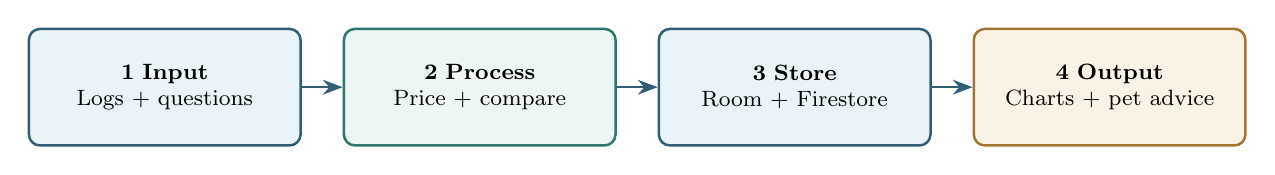
\begin{tikzpicture}[font=\footnotesize,flow/.style={rounded corners=4pt,minimum width=3.45cm,minimum height=1.48cm,text width=3.05cm,align=center,line width=.9pt,inner sep=4pt}]
\node[flow,draw=navy,fill=lightblue] (input) at (1.725,0) {\textbf{1  Input}\\Logs + questions};
\node[flow,draw=teal,fill=lightteal] (process) at (5.725,0) {\textbf{2  Process}\\Price + compare};
\node[flow,draw=navy,fill=lightblue] (storage) at (9.725,0) {\textbf{3  Store}\\Room + Firestore};
\node[flow,draw=amber,fill=lightamber] (action) at (13.725,0) {\textbf{4  Output}\\Charts + pet advice};
\foreach \a/\b in {input/process,process/storage,storage/action}{\draw[-{Stealth[length=2.5mm]},line width=.9pt,draw=navy] (\a.east) -- (\b.west);}
\end{tikzpicture}
\end{center}
Model responses report usage only for calls observed by the caller, so imported Agent logs are the primary input. Java matches token classes to dated prices and computes budgets; the external model receives selected summaries rather than API secrets or prompt text. A server-side function-call loop lets the pet query read-only tools, then return a short recommendation with source and coverage. The pet cannot observe a live coding session without a separate event feed.

\sect{7. Proposed Android interface}
The main navigation has \textbf{Home, Activity, Sessions, Compare and Budget}. Inspired by dsh-context and dsh-pet, these mobile sketches show summary metrics, a heatmap and session cards. The pet floats within the app and opens a question panel on tap; that panel can expand to show evidence. Log-dependent sections show an empty state when records are unavailable.
\vspace{2pt}
\begin{center}
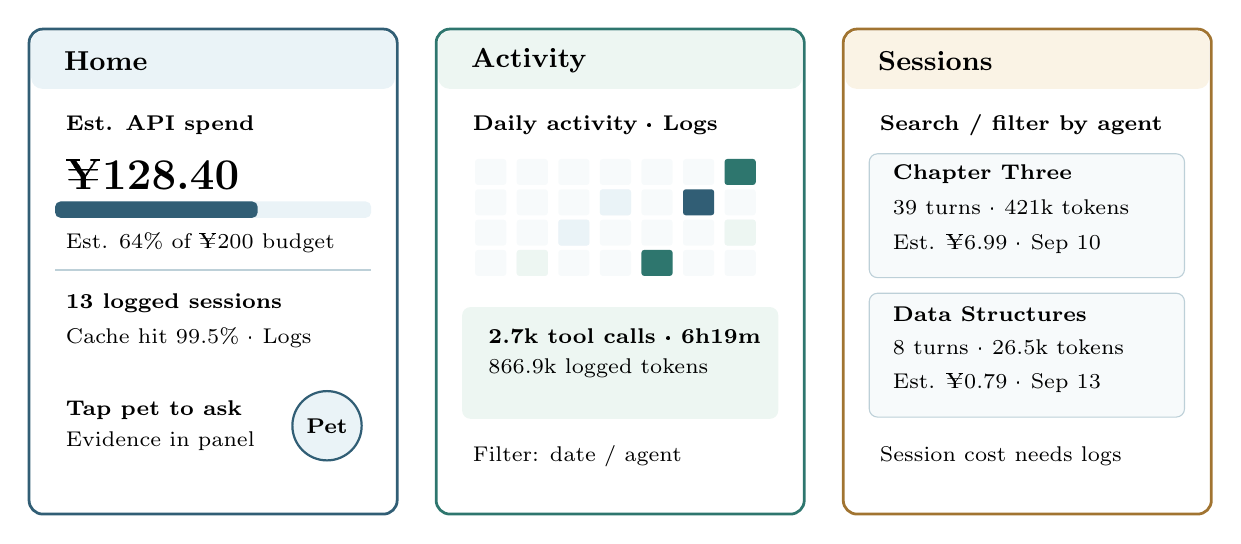
\begin{tikzpicture}[scale=1.1,transform shape,font=\scriptsize,every node/.style={text=black}]
% Three clean screen concepts; colour is limited to borders, fills and data marks.
\foreach \x/\title/\border/\filltone in {0/Home/navy/lightblue,4.7/Activity/teal/lightteal,9.4/Sessions/amber/lightamber}{
  \draw[draw=\border,line width=1pt,rounded corners=5pt] (\x,0) rectangle (\x+4.25,5.6);
  \fill[\filltone,rounded corners=4pt] (\x+.025,4.91) rectangle (\x+4.225,5.575);
  \node[anchor=west,font=\small\bfseries] at (\x+.28,5.23) {\title};
}
% Home: key figure, budget progress and the most urgent next action.
\node[anchor=west,font=\scriptsize\bfseries] at (.3,4.49) {Est. API spend};
\node[anchor=west,font=\Large\bfseries] at (.3,3.92) {¥128.40};
\fill[lightblue,rounded corners=2pt] (.3,3.42) rectangle (3.95,3.61);
\fill[navy,rounded corners=2pt] (.3,3.42) rectangle (2.64,3.61);
\node[anchor=west] at (.3,3.14) {Est. 64\% of ¥200 budget};
\draw[hairline,line width=.5pt] (.3,2.82) -- (3.95,2.82);
\node[anchor=west,font=\scriptsize\bfseries] at (.3,2.44) {13 logged sessions};
\node[anchor=west] at (.3,2.04) {Cache hit 99.5\% · Logs};
\node[anchor=west,font=\scriptsize\bfseries] at (.3,1.20) {Tap pet to ask};
\node[anchor=west] at (.3,.84) {Evidence in panel};
\fill[lightblue] (3.44,1.02) circle (.40);
\draw[draw=navy,line width=.8pt] (3.44,1.02) circle (.40);
\node[font=\scriptsize\bfseries] at (3.44,1.02) {Pet};
% Activity: daily heatmap from dated call or session records.
\node[anchor=west,font=\scriptsize\bfseries] at (5.0,4.49) {Daily activity · Logs};
\foreach \col in {0,...,6}{\foreach \row in {0,...,3}{\fill[lightrow,rounded corners=1pt] ({5.15+0.48*\col},{2.75+0.35*\row}) rectangle ({5.51+0.48*\col},{3.05+0.35*\row});}}
\foreach \col/\row/\tone in {1/0/lightteal,2/1/lightblue,4/0/teal,5/2/navy,6/1/lightteal,6/3/teal,3/2/lightblue}{\fill[\tone,rounded corners=1pt] ({5.15+0.48*\col},{2.75+0.35*\row}) rectangle ({5.51+0.48*\col},{3.05+0.35*\row});}
\fill[lightteal,rounded corners=3pt] (5.0,1.1) rectangle (8.65,2.39);
\node[anchor=west,font=\scriptsize\bfseries] at (5.18,2.05) {2.7k tool calls · 6h19m};
\node[anchor=west] at (5.18,1.68) {866.9k logged tokens};
\node[anchor=west] at (5.0,.67) {Filter: date / agent};
% Sessions: per-session estimates require an authorised agent log.
\node[anchor=west,font=\scriptsize\bfseries] at (9.7,4.49) {Search / filter by agent};
\draw[draw=hairline,fill=lightrow,rounded corners=3pt] (9.7,2.73) rectangle (13.34,4.16);
\node[anchor=west,font=\scriptsize\bfseries] at (9.85,3.92) {Chapter Three};
\node[anchor=west] at (9.85,3.54) {39 turns · 421k tokens};
\node[anchor=west] at (9.85,3.12) {Est. ¥6.99 · Sep 10};
\draw[draw=hairline,fill=lightrow,rounded corners=3pt] (9.7,1.12) rectangle (13.34,2.55);
\node[anchor=west,font=\scriptsize\bfseries] at (9.85,2.31) {Data Structures};
\node[anchor=west] at (9.85,1.93) {8 turns · 26.5k tokens};
\node[anchor=west] at (9.85,1.51) {Est. ¥0.79 · Sep 13};
\node[anchor=west] at (9.7,.67) {Session cost needs logs};
\end{tikzpicture}
\end{center}
\vspace{-2pt}
\smallhead{Interaction and accessibility.} Each screen shows loading, empty and error states. Figures carry Agent, provider, estimate status, usage coverage, price version and refresh time; the heatmap has a numeric summary. A context ring is not API spend. The team checks touch targets, text scaling and screen rotation.

\sect{8. Technology and responsible reuse}
\begin{tabularx}{\linewidth}{@{}>{\raggedright\arraybackslash}p{33mm}Y@{}}
\toprule
\rowcolor{lightblue}
\textbf{Layer} & \textbf{Planned tools and rationale} \\
\midrule
Android interface & Java/XML, Material Components and Navigation; ViewModel/LiveData for state; RecyclerView and MPAndroidChart for trends; an in-app floating pet view and expandable question panel. \\
\rowcolor{lightrow}
Network and work & Retrofit/OkHttp for log import and a Java advice service. The service runs one model API and a bounded function-call loop over read-only usage, budget and comparison tools. WorkManager schedules price checks. \\
Persistence and security & Room plus UID-restricted Firestore; the Java service verifies Firebase ID tokens and holds its model key server-side. Imported metadata is protected; coding-agent passwords and keys are not required. \\
\rowcolor{lightrow}
Open-source reuse & Room with a View guides storage structure; MPAndroidChart may supply charts. dsh-pet inspires interaction, but original or properly licensed art will be used. Reused files and licences will be recorded. \\
\bottomrule
\end{tabularx}

\newpage
\sect{9. Work plan through the final submission}
The three-person team will follow the approximate course checkpoints: Alpha (weeks 8--9), Beta (weeks 11--12) and Final (weeks 15--16). The team will commit to GitHub throughout the project and adjust scope based on tested progress.\par
\begin{tabularx}{\linewidth}{@{}>{\raggedright\arraybackslash}p{24mm}Y >{\raggedright\arraybackslash}p{49mm}@{}}
\toprule
\rowcolor{lightblue}
\textbf{Course weeks} & \textbf{Work} & \textbf{Checkpoint / acceptance} \\
\midrule
1--3 & Confirm API-key Agent use cases and UI, set up Firebase Auth and Firestore rules, document usage-log access and official pricing dimensions. & Neither test account can access the other's records; token-source limits are documented. \\
\rowcolor{lightrow}
4--7 & Implement Agent profiles, usage-log import, Room/Firestore records, versioned pricing, CNY display and dashboard. & Sample calls from each provider are priced with the correct dated rate and de-duplicated. \\
8--9: Alpha & Deliver a working login → add Agent → import token log → estimated cost → analytics path; distinguish real logs from sample data. & Source, description, GitHub link and MP4 demonstration per submission guidance. \\
\rowcolor{lightrow}
10--12: Beta & Add budgets, sessions and task ratings; build the in-app floating pet and tap-to-open panel; connect one model to three read-only tools. & Pet answers a usage question with evidence and admits missing data; test price changes and errors. \\
13--15: Final & Evaluate advice accuracy and API cost, improve accessibility, verify account isolation and document estimation limits. & End-to-end demo and report/video; no pet answer invents usage or controls coding agents. \\
\bottomrule
\end{tabularx}

\sect{10. Team work and evidence of completion}
The team split is \textbf{Zhang Li (24107757)}: UI/UX design, Java/XML screens, charts and accessibility; \textbf{Wang Tingdong (24107759)}: authentication, usage-log import, Room/Firestore, versioned pricing and budget computation; \textbf{Liu Zongrun (24107745)}: in-app floating pet, question panel, external-model service, read-only tools and advice evaluation. All three review integrations and contribute GitHub commits.

The final demo should show: account isolation; tracked Codex, ZCode and DeepSeek-side profiles; three provider estimates from dated token logs; a heatmap and budget warning; then a pet question such as ``Why did cost rise?'' answered with a queried summary, evidence and its own estimated API cost.

Validation will test token accounting, price-version boundaries, missing usage, de-duplication and read-only tool limits; the Firebase Emulator verifies access. Pet replies are checked against tool data. Published rates can differ from paid amounts; all figures remain estimates.

\sect{11. Sources and project references}
\begin{tabularx}{\linewidth}{@{}>{\raggedright\arraybackslash}p{25mm}Y@{}}
\textbf{API scope} & \href{https://developers.openai.com/api/docs/pricing}{OpenAI pricing}; \href{https://api-docs.deepseek.com/quick_start/pricing/}{DeepSeek pricing}; \href{https://docs.z.ai/guides/overview/pricing}{Z.ai pricing}; \href{https://learn.chatgpt.com/docs/auth}{Codex billing modes}; \href{https://zcode.z.ai/en/docs/configuration}{ZCode endpoints}.\\
\textbf{Agent} & \href{https://developers.openai.com/api/docs/guides/function-calling}{Function calling}; \href{https://developers.openai.com/api/docs/libraries}{Java API client}; \href{https://firebase.google.com/docs/auth/admin/verify-id-tokens}{Firebase ID-token verification}.\\
\textbf{Related} & \href{https://github.com/bowenliang123/dsh-context/blob/main/README.md}{dsh-context dashboard}; \href{https://github.com/zhu1090093659/dsh-pet/blob/main/README.zh.md}{dsh-pet}; \href{https://docs.litellm.ai/docs/simple_proxy}{LiteLLM}; \href{https://github.com/android/codelab-android-room-with-a-view}{Room with a View}; \href{https://github.com/PhilJay/MPAndroidChart}{MPAndroidChart}.\\
\textbf{Security} & \href{https://firebase.google.com/docs/firestore/security/rules-conditions}{Firestore Security Rules conditions}.\\
\end{tabularx}

\end{document}
